\documentclass[a4paper,11pt,twoside]{article}
\usepackage[english]{babel}
\usepackage[utf8]{inputenc}
\usepackage{fancyhdr}
\usepackage[margin=1.2in]{geometry}
\usepackage[T1]{fontenc}
\usepackage{ae,aecompl}
\usepackage[parfill]{parskip} 
\usepackage{subcaption} 
\usepackage{graphicx}
\usepackage{bm}
\usepackage{amsmath,amsfonts,mathtools}
\pagestyle{fancy}
\fancyhf{}
\rhead{\textsl{OVERLEAF}}
\lhead{\textsl{GUIDES AND TUTORIALS}}
\renewcommand{\footrulewidth}{0.4pt}% default is 0pt
\fancyfoot[C]{\thepage}
\setcounter{tocdepth}{4}
 
\begin{document}

\tableofcontents
\newpage

\section{Background}
\vspace{6mm}

\subsection{Introduction}

The National Basketball Association (NBA) is a professional basketball league in North America consisting of 30 teams (also called franchises) where each team has of a squad of players called a roster. The teams are evenly split into two `conferences' - the Western Conference and the Eastern Conference. Each team plays 82 games throughout the regular season where they are ranked based off of their win-loss (W-L) record. The top 8 from each conference will then compete in the `playoffs' in an attempt to win the NBA championship. Each franchise is seeded based off of their win-loss record during the regular season and placed in a tournament bracket. Teams with a better win-loss record at the end of the regular season get a higher seeding and are more likely to encounter teams with a lower seeding in the playoffs. In each playoff  round, teams play a best-of-seven game series where the first team to win four games moves into the next round of the playoffs, whereas the other team is eliminated. The championship series occurs when the final two teams left in the playoffs play one another in a seven game series. The team which wins this series are the champions of the NBA season.


\subsection{Project Aim and Motivation}

Player statistics are heavily recorded in the NBA as they are a useful indicator of player performance. After every game individual statistics are recorded for every player allowing franchises and basketball enthusiasts to gain an insight about a players contributions throughout the season. Team and individual stats after each games are summarised by a `box score' see table below. Players are often evaluated using these stat lines and consequently the individual success of a players season can be defined by inferring from their statistics. In the NBA there are a multitude of statistics and metrics that are recorded; a few examples of the most popular metrics recorded are: \textbf{points scored}, \textbf{assists made} and the \textbf{total number of rebounds}. Furthermore it is also possible to see a trend of a players career by observing the information provided by stat lines from their previous games. For example, it can be speculated that a player is improving if their points, assists and total rebounds per game are increasing. As the success of a team is heavily dependent on individual performances from their players, there is a large motivation for franchises to find players who will improve their team. % !! TALK ABOUT + DIAGRAM OF A BOX SCORE!!
\vspace{5mm}
\begin{center}
\scalebox{0.6}{
\begin{tabular}{ |c|c|c|c|c|c|c|c|c|c|c|c|c|c|c|c|c|c|c|c|c|} 
 \hline
 Player & MP & FG & FGA & FG\% & 3P & 3PA & 3P\% & FT & FTA & FT\% & ORB & DRB & TRB & AST & STL &BLK & TOV & PF & PTS & +/-\\ 
 \hline
 Jerami Grant &  &  & & & & & & & & & & & & & & & & & &\\ 
 \hline
 Dennis Schroder &  & & & & & & & & & & & & & & & & & & &\\ 
 \hline
 Russel Westbrook& & & & & & & & & & & &  & & & & & & & &\\
 \hline
 Terrance Ferguson& & & & & & & & & & & &  & & & & & & & &\\
 \hline
 Steven Adams& & & & & & & & & & & &  & & & & & & & &\\
 \hline
\end{tabular}
}
\end{center}
\vspace{5mm}
%PARA BELOW - DISPLAY WHAT MODELS YOU ARE PLANNING MORE CLEARLY!!!!
This project aims to build on previous studies that explore machine learning models for predicting outcomes in the NBA. Moreover, the focus of this project will be experimenting with different statistical and machine learning algorithms starting with a simple average model and moving to more complex models such as non-linear multi-feature regression in order to accurately forecast the points scored by players over the course of the 2018-19 season. More specifically this project will aim to answer the following questions:

\begin{center}
\textbf{Can machine learning models accurately forecast the points scored for players for every game during the 2018-19 NBA regular season using trends from previous seasons?}

and 

\textbf{Can machine learning models accurately forecasting the average points per game of players for the 2018-19 regular season and thus the general trend of a players career?}
\end{center}
\vspace{7mm}

The contributions of this paper can be summarised as follows:
\begin{itemize}
    \item Selecting the best features for the predictive variable - points scored per game
    \item Outlining, analysing and comparing the different machine learning algorithms used.
\end{itemize}
%More emphasis on the TIME SERIES ELEMENT!
Essentially, the project aims to solve a \textbf{time series problem} where outcomes in the future are predicted using information given in the present. \textbf{Is it possible to predict the points scored in future games based off the trend of past games played?}

The NBA is a multi-billion dollar industry that is growing in popularity at a fast rate with viewership numbers reaching a record level in the 2017-18 season. The average franchise value is \$1.9 billion, 13\% more compared to the year prior. Furthermore there is a lot of incentive for franchises to perform well as this would further increase their revenue.

Franchises spend approximately half of their revenue on player salary, and in many ways, risk their monetary success on the future of their players when signing them for multi-million dollar long-term contracts. Such monetary risks include team success over multiple seasons, salary cap restrictions, overall franchise value and team marketability. As a result, the necessity for franchises to accurately forecast future player performance has increased greatly over the recent years in order to acquire players that will aid the teams success.

The main motivation for this project is to help NBA franchises make more informed and well judged decisions when attempting to acquire players. Coaches, scouts and agents can use the models explored  to forecast a particular player?s future performances and monitor their development before deciding whether or not to acquire the player. 

Another motivation for exploring this project is the drastic increase in the sports analytics industry and its role in the sports betting market. The sports analytics market is expected to reach \$2.09 billion by 2022, with many more basketball enthusiasts exploring different methods to predict outcomes in basketball games. For example Google Cloud, NCAA and Kaggle hosted the annual `March Madness' competition where basketball fans attempt to forecast outcomes of a college basketball tournament in an attempt to win up to \$10,000.

 Furthermore the sports betting market is so large solely because it is challenging to predict the outcomes of sporting events. As a result, another motivation for exploring this project is to discover a more accurate method of predicting player outcomes to better inform sports betting enthusiasts. 



\subsection{Existing Literature}
 
\subsubsection{ARIMA model Time Series Player Data}

%NEED TO PROOF-READ + MAKE SURE IT MAKES SENSE - potensh add mathematical formulae
This paper explores game-by-game data of one player, Derrick Rose, in order to forecast the number of points scored in upcoming games. More specifically this paper attempts to find the best ARIMA model that best fits Derrick Rose?s previous statistics in order to accurately predict Rose?s future points per game. 

The paper uses data from the 2014-15 regular season and as a result the ARIMA models used  were trained using only 51 games of the season (Rose only played 51 games of the regular season, the other 31 were missed due to injury).

ARIMA(p,d,q) stands for Autoregressive Integrated moving average and is commonly used in time series analysis where the data displays non-stationary properties, that is the mean and variance changes over time. This model is a generalisation of the ARMA(p,q) model, which combines the autoregressive model with the moving average model. The autoregressive model (AR(p)) learns from the previous ?p? games played and uses them as inputs for a regression model to predict the points scored in future games. The moving average (MA(q)) model essentially takes the average of the previous ?q? data points. The ?integrated? part of the ARIMA(p,d,q) model consists of finding the differences between ?d? data points in order to remove the non-stationary element.

The motivation behind using the ARIMA model is that DeLay assumed there would not be a seasonal trend over the course of the year and as a result the mean and variance of points scored over the course of the season would not change. Another assumption made was that the forecasted points scored by Rose in future games would be similar compared to his previous games implying that there would be no drastic improvement or deterioration in points scored by Rose in the near future.

The results produced in this paper suggest that an an integrated moving average of order 1 (IMA(1,1)) best fit Derrick Rose?s training data, however the forecasted data was slightly inconclusive. The predicted data points over the next 31 games converged to the average of the initial 51 data points. This was potentially due to the fact that the training data set was too small. Delay believed that over time and given more data, the model would predict more fluctuating data points before averaging out at at slower pace. 

%DOESNT MAKE MUCH SENSE RN, NEEDS A PROOF READ BADLY!!

\subsubsection{Weibull-Gamma Statistical Model}

Hwang et al (2012) attempted to forecast the trend of a small subset (7) of player?s careers using a different statistical method, namely the Weibull-Gamma model. More specifically, Hwang attempted to forecast the average points per game (PPG) scored by players over the upcoming seasons. The subset of players were all ?free agents?, meaning they were currently not under contract with any particular team in the NBA. This paper aimed to aid NBA franchises such that they could obtain a degree a foresight when deciding whether sign these free agents.


Before deciding to use average PPG over a season as a method for evaluating player performance an array of different features were experimented with to find an accurate metric for player performance. Hwang?s reasoning for using the average PPG over the course of a season was because it is a very commonly used statistic. As a result the training data consisted of seven different players, the target variable was the average PPG for a season and the dependent variable was the season number. 

The statistical model used was a mixture of the Weibull-hazard and the gamma function. The motivation behind using this model is that the assumption of performance over time is included. In other words, Hwang assumes that player performance will begin to decline as the players partake in more NBA seasons and therefore he is expecting the average points scored per game to decline as more seasons occur.

The results achieved by Hwang after one season of predicting the average PPG for the season upcoming (2010-11) season were fairly encouraging. The difference in points never exceeded more than 2, proving to be a fairly accurate model.

A key difference between Hwang?s thesis and the objective in this thesis is that Hwang does not attempt to predict the points scored for individual games throughout a season, only the average points scored per game over the entire season. Therefore it can be deduced that this study was focused more on forecasting the general trend of player careers, attempting to decipher the effect of age on a players career rather than attempting to predict the points per game of a player against a particular team

\subsection{The Dataset}

This investigation will focus on a specific subset of players, specifically players from the 2014 Draft Class. The dataset consists of 27 players and their box score statistics of every game from the previous three seasons. The players and the the references to the statistics are shown below. The incentive for choosing these players is:
\begin{itemize}
    \item These players are of similar ages and they have had the same number of years of experience in the NBA.
    \item They are still relatively young, so the possibility of a decline in performance due to aging is low.
    \item Although these players are still relatively young, they have played 3 seasons in the league and therefore they should be well adjusted to the difficulty of the NBA.
\end{itemize}
Therefore the assumption made when using this dataset is that it is unlikely that the performance of these players is unlikely to drastically improve or decline over the course of the 18/19 season and therefore these players points per game may be more predictable.

The data was collected by scraping the box scores off of the website BasketBall Reference. Some box score statistics can be see as good indicators for predicting future points per game and as a result can be considered as important features. The box score statistics are explained in Table XX.

\vspace{5mm}
\begin{center}
\begin{tabular}{ ccccc } 
 \hline
Andrew Wiggins & Jabari Parker & Joel Embiid & Aaron  Gordon& Dante Exum \\ 
 \hline
Marcus Smart & Julius Randle & Nik Stauskus & Noah Vonleh & Elfrid Payton \\ 
 \hline
 Doug McDermott & Zach LaVine & T.J Warren & Jusuf Nurkic & Gary Harris\\
 \hline
 Bruno Caboclo & Rodney Hood & Shabazz Napier & Clint Capela & Kyle Anderson\\
 \hline 
 Joe Harris & Spencer Dinwiddie & Jerami Grant & Glenn Robinson & Nikola Jokic\\
 \hline
  Dwight Powell & Jordan Clarkson\\
\hline
\end{tabular}
\end{center}

 \subsubsection{Overview of the Features}
The box scores from every game over the past 3 seasons  were scraped from ?Basketball Reference? (see Figure 1 for an example of a box score). The stats recorded could potentially be used a features for forecasting points per game for future games. The features (and the target variable) provided are summarised in the following table. 

\vspace{5mm}
\begin{center}
\begin{tabular}{ |c|c| } 
 \hline
MP & Minutes Played  \\ 
 \hline
FG & Field Goals scored \\ 
 \hline
FG\% & Field Goal percentage\\ 
 \hline
3P & Number of 3 point field goals\\
 \hline
 3P\% & 3 point field goal percentage\\
\hline
FT & Number of free throws made\\
\hline
FTA & Number of free throws attempted\\
\hline
FT\% & Free throw percentage\\
\hline
ORB & Number of offensive rebounds\\
\hline
DRB & Number of defensive rebounds\\
\hline
TRB & Total number of rebounds\\
\hline
AST & Number of assists made\\
\hline
STL & Number of steals made\\
\hline
BLK & Number of blocks made\\
\hline
TOV & Number of turnovers conceded\\
\hline
PF & Number of personal fouls conceded\\
\hline
PTS & Number of points scored\\
\hline
+/- & Net number of points scored when on the court\\
\hline
\end{tabular}
\end{center}
\vspace{5mm}


There are other factors which could determine the number of points scored by a player in a game which are not captured using just box score statistics. One of these factors is ?player form?. This can often be hard to quantify, as there is not statistic in basketball which tell us how well a player is performing.  However, a potential way to include form would be use a rolling-window of points scored from previous games, and use this as a feature for predicting the points scored for the upcoming game.  Additionally, another main factor not included in box scores is opponent difficulty. The motivation for including opponent difficulty is that teams vary in defensive capabilities which could impact how many points a player scores in a game.


\subsection{Feature Selection Methods}
In order to improve the performance of the models when predicting the target variable, the most relevant features need to be selected. Feature selection is the approach of selecting the most relevant features for predicted the target variable. Feature selection is used because it removes the features which are irrelevant when predicting the target variable and it aids in avoiding the curse of dimensionality. Additionally feature selection enhances generalisation by reducing overfitting. As Table X shows, there are many features present, however there are some features which may not be pertinent to forecasting the desired target variable, points scored. As a result, different feature selection algorithms were explored, namely the 'SelectKBest' algorithm.


\subsubsection{Select K Best Algorithm}
The SelecKBest algorithm selects a subset of features of size k which have the strongest relationship with the target variable. A wide range of statistical tests can be used to select these features. The statistical test produces a score for each feature, and the top ?k? features which have the highest score the features which have the strongest relationship with the target. For example, a common statistical test used for this algorithm is the chi-squared statistical test.  

 \subsubsection{Feature Importance Using the Extra-Trees Classifier}
 Hello,  here  is  some  text  without  a  meaning.   This  
text  should  show  what  a printed text will look like at 
this place.  If you read this text, you will get no information.  
Really?  Is there no information?  Is there a difference between 
this ... 


% MAYBE PUT ML ALGOS AFTER INTRODUCING THE DATA SET + FEATURES STUFF
\subsection{Technical Background}
%+ the theory of fitting models to dat aand avoiding overfitting and such!
The following section outlines the theory of the machine learning models used in this project. In addition, the motivation and assumptions made when using these models will also be highlighted:


\subsubsection{Simple Moving Average}
The moving average model is commonly used in time series data. The simple average model essentially uses the previous ?n? data points to forecast future data points by taking the unweighted mean of these ?n? points:
\begin{equation}
\bar{p}_{SMA} = \frac{p_{M} + p_{M-1} + ... + p_{M-(N-1)}} {n} 
= \frac{1}{n} \sum_{i=0}^{n-1}p_{M-i}
\end{equation}

In regards to forecasting points scored by players, the simple moving average assumes that the points scored in the previous ?n? games will be enough information to forecast points scored in the 18/19 NBA Season. The simple average model also assumes that a player will score the exact same number of points for every game of the upcoming season, which can be interpreted as a naive assumption.


\subsubsection{Simple Linear Regression}
Ordinary Least Squares (OLS) or Linear Regression is a linear approach to modelling the relationship between an explanatory variable and the target variable.  Given explanatory variable \(x\) and target variable \(y\), the linear relationship is defined as follows:
\begin{equation}
y(x,w) = w_{0} + w_{1}x
\end{equation}
\textbf{w} (the weight vector) encodes the relationship between the two variables. Simple linear regression attempts to best fit a line to a set of data points by finding values for \textbf{w} which minimises the sum of the squares of the vertical offsets of the points from the line. Essentially the aim is to minimise the following function:
\begin{equation}
L(x) = \sum_{i=0}^{n}(y_{i}-\textbf{w}^Tx_{i})^2
\end{equation}
Where $\textbf{w}^Tx_{i}$ is a point on the line  and \(y_i\) is the data point that is vertical offset from  $\textbf{w}^Tx_{i}$. In order to minimise this function the partial derivative of $L$ is taken and the following derivative is equated to 0. As a result, the following equations encode the values of \(w_{0}\) and \(w_{1}\) which best fit the data points:
\begin{equation}
w_{1} =\frac{\sum{}^{} (x_{i} - \bar{x})(y_{i} - \bar{y})}{\sum{}^{}(x_{i} - \bar{x})^2}
\end{equation}
\begin{equation}
w_{0} = \bar{y} - w_{1}\bar{x}
\end{equation}
where $\bar{y}$ and $\bar{x}$  are the means of the $y$ values and $x$ values.

Concerning this investigation, the target variable will be points scored per game and the explanatory variable will be the game number. Furthermore, simple linear regression will produce a linear trend between the number of games played in the NBA and the points scored per game. As a result, when attempting to forecast the points scored games in the upcoming 2018/19 season, the model will work under the assumption that the points scored in every following game will follow a linear trajectory resembling the trajectory of the fitted line produced from training data (previous seasons).

\begin{figure} [h!]
  \centering
  \begin{subfigure}[b]{0.4\textwidth}
    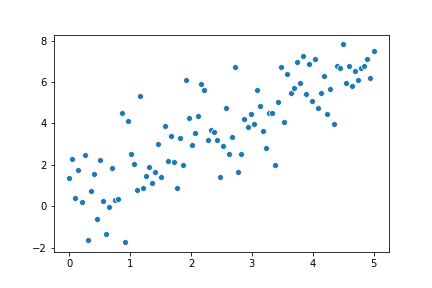
\includegraphics[width=\textwidth]{scatterplt_ex.png}
    \caption{Data Points Plotted}
    \label{fig:1}
  \end{subfigure}
  %
  \begin{subfigure}[b]{0.4\textwidth}
    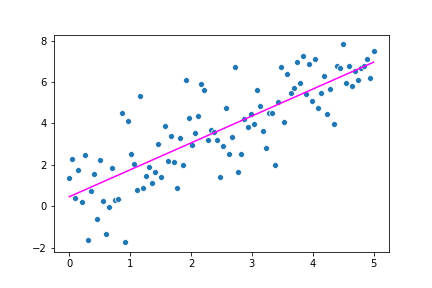
\includegraphics[width=\textwidth]{linregscatterplt.png}
    \caption{Linear Relationship calculated}
    \label{fig:2}
  \end{subfigure}
  \caption{An example of Linear Regression}
  \label{fig:3}
\end{figure}

\subsubsection{Bayesian Linear Regression}
% improve description of theory for Bayesian LS
Bayesian Linear Regression also formulates a linear relationship between the explanatory and target variables, however unlike OLS the relationship is based off a probability distribution rather than point estimates. In other words, the target value is not estimated to be a single value but it is drawn from a specific probability distribution. For this investigation, the weights will be sampled from a Gaussian distribution when computing the target values. The reasoning behind this stems from the Central Limit Theorem. Bayesian linear regression uses Bayes Theorem to produce probability distribution for the target values, this probability distribution is called the posterior. A probability encoding an existing or prior belief of the weights (also called parameters) is multiplied by the likelihood of the data points. It is then divided by a normalisation constant. The prior belief will be a Gaussian Distribution, and due to conjugacy, the posterior will also follow a Gaussian Distribution. 
\begin{equation}
 y \sim N(\textbf{w}^T\textbf{X}, \sigma^2\textbf{I})
\end{equation}
\begin{equation}
P(\textbf{w}|y,\textbf{X}) = \frac{P(y|\textbf{X},\textbf{w})P(\textbf{w})}{P(y|\textbf{X})}
\end{equation}
One of the benefits of using Bayesian linear regression is that a prior belief about the model parameters can be specified, rather than assuming that all the information regarding the parameters is included within the data set. Another benefit of Bayesian linear regression is that uncertainty is included in our model due to the fact that the posterior is a probability distribution. If the dataset is small the posterior distribution of the parameters will be more spread out. Therefore it can be implied that the model is more uncertain in its belief of parameter values. As more data points are observed the posterior probability is ?updated? and the model becomes more certain concerning its parameter values. If infinite data points were to be observed, the prior probability would essentially be washed out, and the best fitting line would converge to the OLS best fitting line.

The main motivation for including this model in this investigation is that a prior belief about the trajectory a particular player?s upcoming season. (expand on this later)

\subsubsection{Kernel Ridge Regression}
%TEMPORARY - GET RID OF THIS LATER
Kernelised Ridge Regression is a nonlinear approach for modelling the relationship between an explanatory variable and a target variable. It combines Ridge Regression with the ?kernel trick?.

Ridge Regression is similar to least squares regression where a curve is best fitted to a set of data points through minimising a loss function specified by Equation (2). However, the major risk when attempting to fit a curve to data is overfitting. One simple method for avoiding overfitting is to include penalty term to w in the loss function. The loss function becomes, 
\begin{equation}
L = \sum_{i=0}^{n}y_{i} - \textbf{w}^Tx_{i} + \lambda||\textbf{w}||^2
\end{equation}
$\lambda$ is the regularisation parameter. If $\lambda$ were to be zero, then the loss function function would be the same as the loss function for least squares.

\begin{figure} [h!]
  \centering
  \begin{subfigure}[b]{0.4\textwidth}
    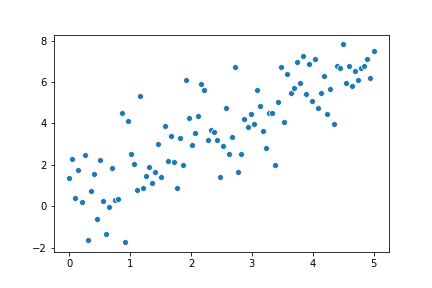
\includegraphics[width=\textwidth]{scatterplt_ex.png}
    \caption{Data Points Plotted}
    \label{fig:1}
  \end{subfigure}
  %
  \begin{subfigure}[b]{0.4\textwidth}
    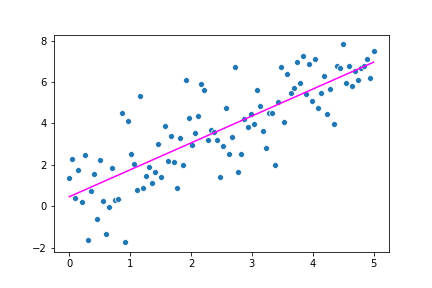
\includegraphics[width=\textwidth]{linregscatterplt.png}
    \caption{Linear Relationship calculated}
    \label{fig:2}
  \end{subfigure}
  \caption{An example of Linear Regression}
  \label{fig:3}
\end{figure}

In order to achieve a nonlinear curve a kernel function, $k(x,x')$ is applied to all input values. Kernel functions describe the inner product of two input values that are mapped to a different feature space $\mathcal{X} \rightarrow \mathcal{F}$: $k(x_{1},x_{2}) = \phi(x_{1})^T\phi(x_{2})$. The basis function $\phi(.)$ is unknown however it is not required as long as the mapped feature space is an inner product space; this is known as the kernel trick The idea behind using kernels is that when the inputs are mapped to a different feature space, they can be classified linearly as seen in Figure X. Examples of kernel functions include the Radial Basis Function, the Polynomial Kernel and the  Fisher Kernel.

      \begin{figure}[!htb]
        \center{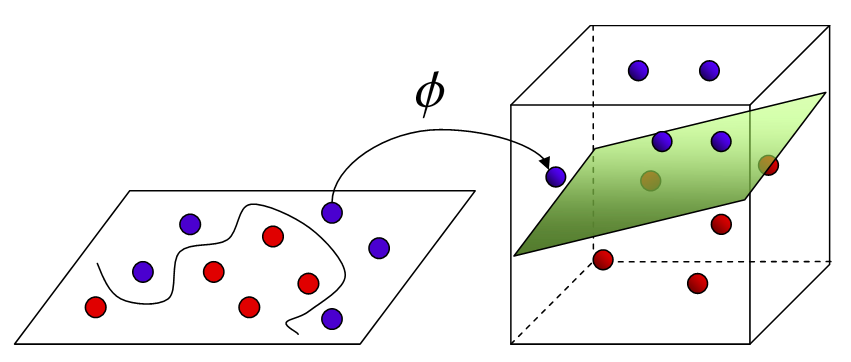
\includegraphics[width=0.5\textwidth]
        {kerneltrick.png}}
        \caption{\label{fig:my-label} My figure.  An example of a cool figure}
      \end{figure}

The main motivation behind using Kernel Ridge Regression in this investigation is that the trajectory of a players performance over games played may not be linear. For example, a number of points scored by a player may have improved exponentially over last 20 games, and therefore applying a non-linear curve to this data may better fit the trajectory of his career. It can be inferred that this model will place more emphasis on recent form when attempting to forecast future results.
\begin{figure} [h!]
  \centering
  \begin{subfigure}[b]{0.32\textwidth}
    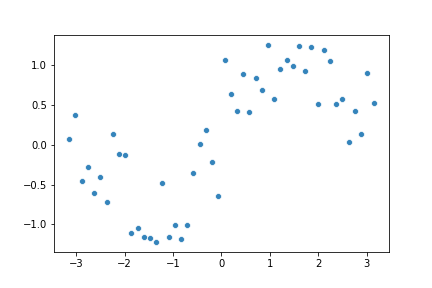
\includegraphics[width=\textwidth]{wavey.png}
    \label{fig:4}
  \end{subfigure}
  %
  \begin{subfigure}[b]{0.32\textwidth}
    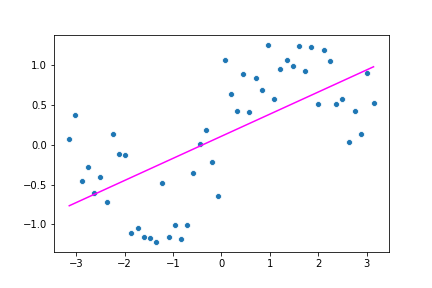
\includegraphics[width=\textwidth]{wavey_lr.png}
    \label{fig:5}
  \end{subfigure}
  %
  \begin{subfigure}[b]{0.32\textwidth}
    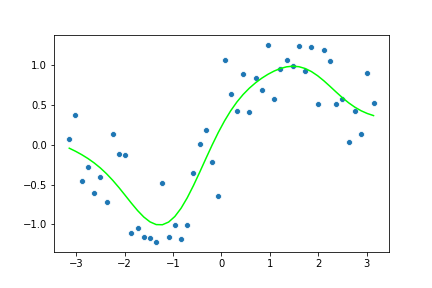
\includegraphics[width=\textwidth]{wavey_kr.png}
    \label{fig:6}
  \end{subfigure}
  \label{fig:7}
\end{figure}

\subsubsection{Multiple Linear Regression and Multivariable Kernel Ridge Regression}

Multiple Linear Regression models a relationship between more than one explanatory variable and a target variable by fitting a linear equation to the observed data:
\begin{equation}
y_{i} = w_{0} + w_{1}x_{i} + w_{2}x_{i} +  ... + w_{n}x_{i}
\end{equation}
A feature matrix consisting of the explanatory variables $\textbf{X}$ and a column vectors consisting of the target variable $y$ and weights $\textbf{w}$ can be represented as:
\[
\begin{bmatrix}
    x_{11} & x_{12} & x_{13} & \dots  & x_{1n} \\
    x_{21} & x_{22} & x_{23} & \dots  & x_{2n} \\
    \vdots & \vdots & \vdots & \ddots & \vdots \\
    x_{d1} & x_{d2} & x_{d3} & \dots  & x_{dn}
\end{bmatrix}
\]
In order to establish a linear relationship between $y$ and $\textbf{X}$ the weights are calculated using the least squares method akin to simple linear regression. Therefore the following loss function that needs to be minimised is Xw -y 2. The formula for finding the weights which minimise Equation X is
\begin{equation}
\textbf{w} = (\textbf{X}^T\textbf{X})^{-1}\textbf{X}^Ty
\end{equation}
Within the context of this investigation, multiple linear regression allows for different features other than just games played over time. For example, if a player is playing against a team who is less defensively adept compared to other teams, the player may score more points in that particular match compared to the other teams, or a player may have recently hit a good patch of form over the past few games, it is therefore logical to assume he will score more points in the next game. Using more features may allow for a more accurate prediction of player points per game. Multiple Linear Regression assumes that each explanatory variable is independent from another.

Multivariable Kernel Ridge Regression is a simple extension of its single feature counterpart. Additionally, like Multiple linear regression  there is or than one explanatory variable describing the target variable. 

 \subsubsection{Training and Test Data}
Machine learning models are initially fit on a training dataset. The training data consists of a set of explanatory variables and the respective target variables. The model essentially learns from this data and fits its parameters to the training data. After the model is trained, its performance is assessed using a test dataset. If the models performance of the training data is is similar to that of the test data.

\subsubsection{Overfitting}
When attempting to fit a machine learning model to data, it is important that overfitting is avoided. Overfitting occurs when the machine learning algorithm attempts to learn the noise within the dataset as well as attempting to learn the signal presented in the dataset. Noise in a dataset refers to the randomness within a dataset and signal refers to the underlying pattern in the dataset that wish to learn.One approach of detecting overfitting when learning is to plot the validation error of the training data and the test data. If the validation error begins to increase for the test data while decreasing for the training data then the model has most likely over fitted the training data. 

      \begin{figure}[!htb]
        \center{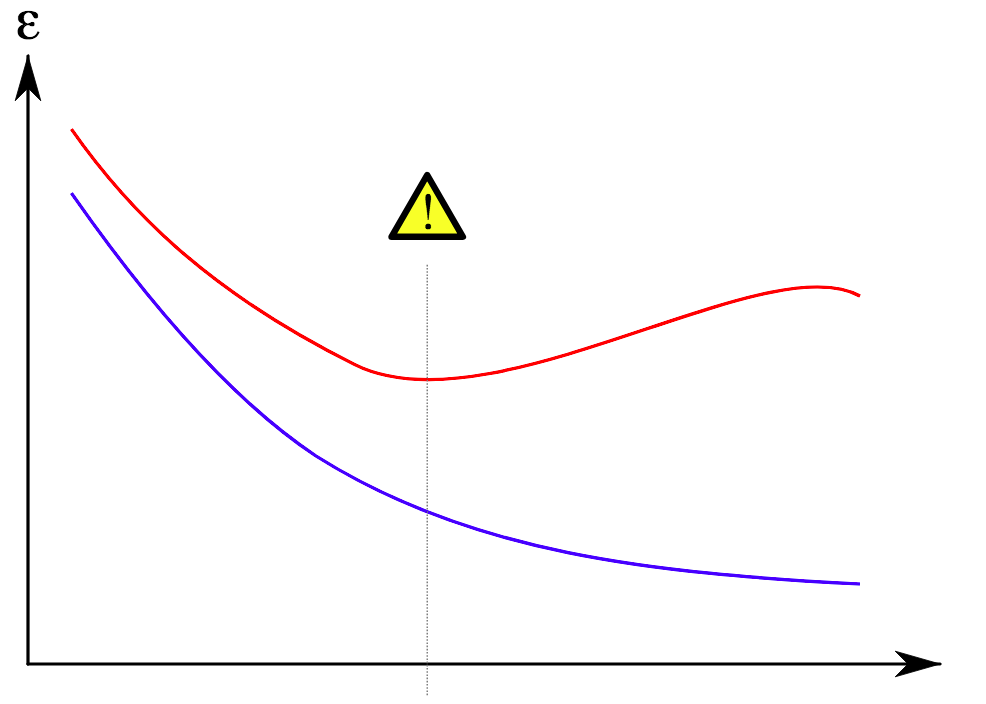
\includegraphics[width=0.5\textwidth]
        {overfitpng.png}}
        \caption{\label{fig:my-label} My figure.  An example of a cool figure}
      \end{figure}

\subsubsection{Root Mean Squared Error}
This investigation will use the Root Mean Squared Error (RMSE) quantify the error in each model. RMSE is that standard deviation between the values predicted by a machine learning model and the values observed.
\begin{equation}
RMSE = \sqrt[]{\frac{\sum_{i=0}^{n}(\hat{y}_{i} - y_{i})}{n}}
\end{equation}
In order to check whether a model has over fit or underfit the data, the RMSE from the training data and the RMSE of the test data will be compared. If the RMSE is drastically higher for the test data compared to the training data then the model has over fit the data. If the RMSE for both sets are similar then the model has fit the data well. 

Additionally, the RMSE can be used to compare the efficacy between models. Models with a lower RMSE compared to others imply that they?re better at forecasting the trajectory of player points per game compared to models which score a higher RMSE.



\newpage

\section{Methodology and Implementation}

\subsection{Feature Selection}

\begin{figure} [h!]
  \centering
  \begin{subfigure}[b]{0.4\textwidth}
    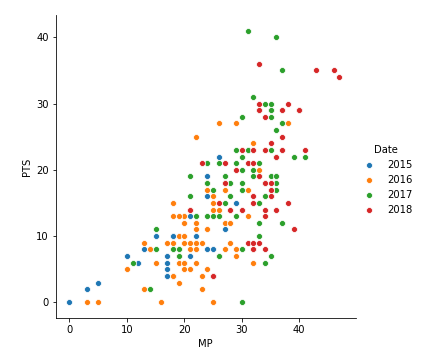
\includegraphics[width=\textwidth]{pairplot1.png}
    \caption{Data Points Plotted}
    \label{fig:1}
  \end{subfigure}
  %
  \begin{subfigure}[b]{0.4\textwidth}
    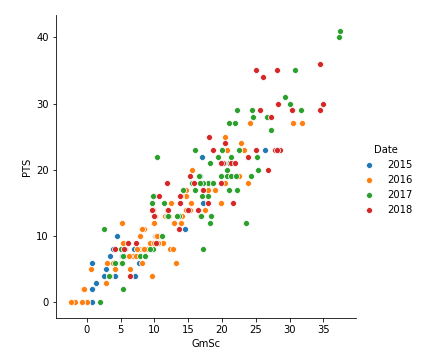
\includegraphics[width=\textwidth]{pairplot2.png}
    \caption{Linear Relationship calculated}
    \label{fig:2}
  \end{subfigure}
  \caption{An example of Linear Regression}
  \label{fig:3}
\end{figure}

\begin{figure} [h!]
  \centering
  \begin{subfigure}[b]{0.4\textwidth}
    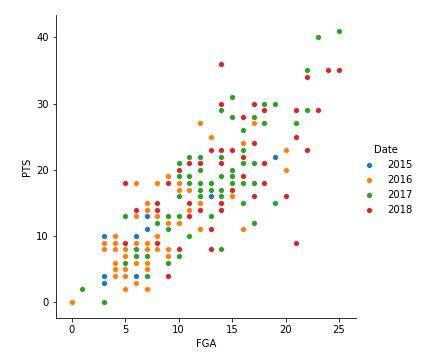
\includegraphics[width=\textwidth]{pairplot3.png}
    \caption{Data Points Plotted}
    \label{fig:1}
  \end{subfigure}
  %
  \begin{subfigure}[b]{0.4\textwidth}
    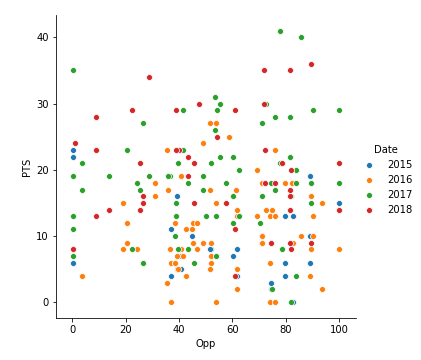
\includegraphics[width=\textwidth]{pairplot4.png}
    \caption{Linear Relationship calculated}
    \label{fig:2}
  \end{subfigure}
  \caption{An example of Linear Regression}
  \label{fig:3}
\end{figure}

\begin{figure} [h!]
  \centering
  \begin{subfigure}[b]{0.45\textwidth}
    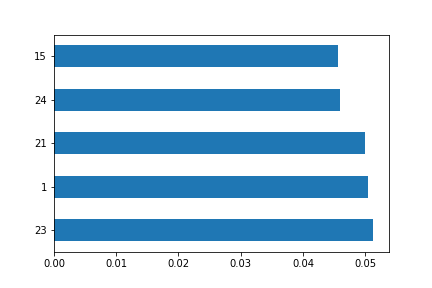
\includegraphics[width=\textwidth]{extratreeclf.png}
    \caption{Data Points Plotted}
    \label{fig:1}
  \end{subfigure}
  %
  \begin{subfigure}[b]{0.45\textwidth}
    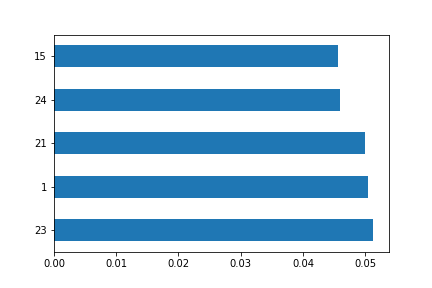
\includegraphics[width=\textwidth]{extratreeclf.png}
    \caption{Linear Relationship calculated}
    \label{fig:2}
  \end{subfigure}
  \caption{An example of Linear Regression}
  \label{fig:3}
\end{figure}

\begin{figure} [h!]
  \centering
  \begin{subfigure}[b]{0.45\textwidth}
    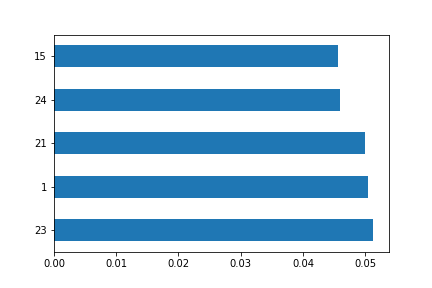
\includegraphics[width=\textwidth]{extratreeclf.png}
    \caption{Data Points Plotted}
    \label{fig:1}
  \end{subfigure}
  %
  \begin{subfigure}[b]{0.45\textwidth}
    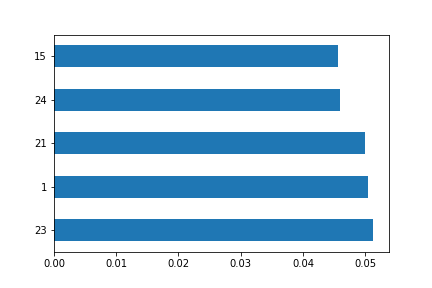
\includegraphics[width=\textwidth]{extratreeclf.png}
    \caption{Linear Relationship calculated}
    \label{fig:2}
  \end{subfigure}
  \caption{An example of Linear Regression}
  \label{fig:3}
\end{figure}



\end{document}